\documentclass[10pt,a4paper]{article}
\usepackage[margin=2.2cm]{geometry}
\usepackage{fontspec}
\usepackage{kotex}
\setmainfont{Apple SD Gothic Neo}
\setsansfont{Apple SD Gothic Neo}
\usepackage{amsmath,amssymb}
\usepackage{graphicx}
\usepackage{booktabs}
\usepackage{caption}
\usepackage[dvipsnames]{xcolor}
\usepackage[colorlinks=true,linkcolor=MidnightBlue,citecolor=MidnightBlue,
            urlcolor=MidnightBlue]{hyperref}
\usepackage{titlesec}
\titleformat{\section}{\large\bfseries}{\thesection}{0.6em}{}
\titleformat{\subsection}{\normalsize\bfseries}{\thesubsection}{0.5em}{}
\captionsetup{font=small,labelfont=bf}
\setlength{\parskip}{0.35em}
\setlength{\parindent}{0pt}

\usepackage{mdframed}
\newmdenv[linewidth=0.4pt,linecolor=gray!60,backgroundcolor=gray!5,
          innertopmargin=6pt,innerbottommargin=6pt,skipabove=8pt,skipbelow=8pt]{claimbox}
\newcommand{\claim}[2]{\begin{claimbox}\textbf{주장.} #1\par\smallskip
  \textcolor{gray!70}{\textbf{반증 조건.} #2}\end{claimbox}}

\title{\bfseries 서랍에 넣는다\\[2pt]
\large 뽑기를 셋에서 여섯으로 늘리니 전이가 $23\%$ 줄었다 --- 그리고 한 시간 전 내
헤드라인이 이상치였다}
\author{월드모델 실험실 · 노트 782 $\sim$ 785}
\date{2026-08-07}
\begin{document}\maketitle

\section{한 줄}

논문 $155$ 가 만화 세 열의 \textbf{집안 통과}를 얻었다(신호 몫 $+0.0231$). 규약 $12$ 가
채택에 \textbf{집 밖 $\geq 2$} 를 요구하므로 KR 만화($1{,}716$행) · CN 만화($352$행)에서
쟀다.

\textbf{집 밖 $0/2$ 다.} KR $\Delta$ $\mathbf{+0.0177}$(문턱 $0.025$ 의 $70.6\%$) ·
CN $\Delta$ $+0.0078$(문턱 $0.022$ 의 $35\%$). \textbf{채택하지 않고 서랍에 넣는다.}

\textbf{그리고 한 시간 전 내 헤드라인이 이상치였다} --- 뽑기 셋으로는 KR $\Delta$ 가
$+0.0230$ 이어서 \emph{``집안 $+0.0231$ 이 크기를 유지했다''}고 적었는데, \textbf{뽑기
여섯에서는 $+0.0177$ 로 $23\%$ 줄었다.}

\section{배선은 완벽했다}

\begin{center}
\begin{tabular}{ll}
\toprule
판 만화 & $5{,}905$행 $=$ 축 파일 $5{,}905$행 \\
사상 & \textbf{판(JP)에서 배워 짝에 적용}(\texttt{mg\_format} $3$범주 · \texttt{mg\_adult}
$2$범주 · \texttt{mg\_nauthor} JP $5{,}905$값 경험분포) \\
짝 행수 & KR $\mathbf{1{,}716}$ · CN $\mathbf{352}$ --- \textbf{시험 ① 통과} \\
짝의 $3$열 마스크 & $1.0 \cdot 1.0 \cdot 1.0$ --- \textbf{조용한 중립화 없음} \\
\bottomrule
\end{tabular}
\end{center}

\textbf{두 함정을 미리 적고 지켰다.} ① \texttt{pairs.to\_arrays} 는 짝 행에 없는 열을
\textbf{$0.5$ · 마스크 $0$} 으로 채운다 --- 그래서 새 $3$열을 \textbf{짝 행에도
붙였다}(안 붙이면 ``안 통한다''와 ``열이 없다''가 구분되지 않는다). ② 사상을 짝에서
다시 계산하면 \textbf{다른 축}이 되므로 \textbf{판에서 배워 적용}했다.

\subsection*{시험 ② --- KR 은 통과, CN 은 실패}

\begin{center}
\begin{tabular}{lrrl}
\toprule
& 실측 & 기록 & 차 \\
\midrule
KR 만화 & $0.6831$ & $0.6841$ & $\mathbf{0.001}$ --- \textbf{통과} \\
CN 만화 & $0.3874$ & $0.3094$ & $\mathbf{0.078}$ --- \textbf{실패} \\
\bottomrule
\end{tabular}
\end{center}

\claim{\textbf{\texttt{lab/pairs.py} 가 이것을 미리 적어 뒀다.} 그 모듈의 경고가
\emph{``CN 은 이 빌더에서 \texttt{entry\_friction} 이 상수라 강등된다 $\ldots$ 그 차이가
기준선을 못 맞추는 첫 후보다(노트 $683$ 예측)''}였다. \textbf{예측이 맞았다} --- 그래서
CN 의 절대 rho 는 기록된 숫자와 견주지 않는다(노트 $579 \cdot 580$).}
{그 경고가 있었으니 \textbf{CN 을 아예 쓰지 말았어야 했나} --- 그러면 집 밖이 하나뿐이라
규약 $12$ 를 애초에 못 만족한다. \textbf{그것이 이 축의 구조적 한계}이고 미리 적어야
했다: \textbf{만화 구조 열은 집 밖 짝이 둘뿐이고 그중 하나는 기준선이 어긋나 있다.}}

\begin{figure}[t]\centering
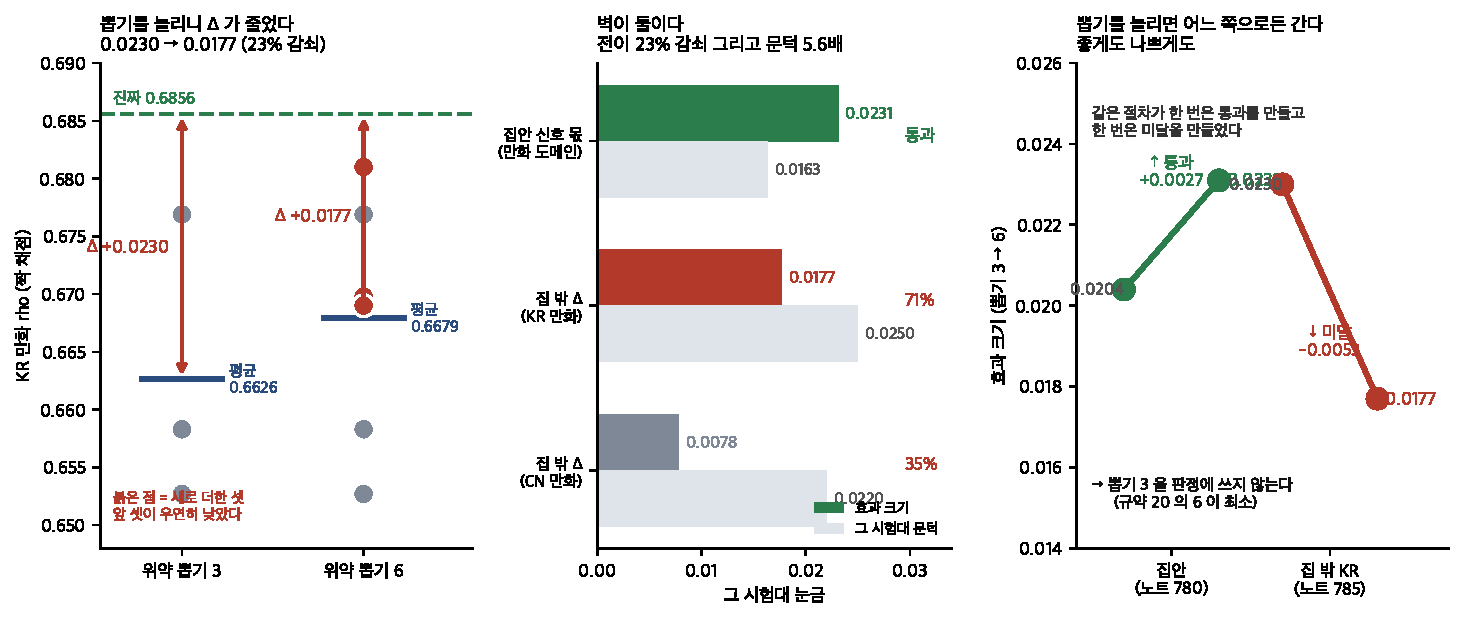
\includegraphics[width=0.99\textwidth]{figs/drawer.pdf}
\caption{왼쪽: \textbf{뽑기를 늘리니 $\Delta$ 가 줄었다} --- 앞 셋이 우연히 낮았다.
가운데: \textbf{벽이 둘이다} --- 전이 감쇠와 문턱. 오른쪽: \textbf{뽑기를 늘리면 어느
쪽으로든 간다}.}
\end{figure}

\section{결과 --- 집 밖 $0/2$}

\begin{center}
\begin{tabular}{lrrrrl}
\toprule
짝(행) & 없이 & 진짜 & 위약 평균 & $\Delta$ & 문턱 \\
\midrule
KR 만화($1{,}716$) & $0.6831$ & $\mathbf{0.6856}$ & $0.6679$(뽑기 $6$) & $\mathbf{+0.0177}$ & $0.025$ --- $70.6\%$ \\
CN 만화($352$) & $0.3874$ & $0.3898$ & $0.3820$(뽑기 $3$) & $+0.0078$ & $0.022$ --- $35\%$ \\
\bottomrule
\end{tabular}
\end{center}

KR 위약 여섯: $0.6527 \cdot 0.6769 \cdot 0.6583 \cdot 0.6698 \cdot 0.6810 \cdot
0.6690$(평균 $0.6679$ · 뽑기 SD $0.01078$ · 폭 $0.0283$). \textbf{진짜가 여섯 전부보다
크지만}($6/6$) \textbf{문턱을 못 넘는다.}

\section{한 시간 전 내 헤드라인이 이상치였다}

노트 $783$ 이 뽑기 셋으로 KR $\Delta$ $+0.0230$ 을 얻고 \textbf{가장 중요한 숫자}로
이렇게 적었다: \emph{``집안 $+0.0231$ 이 KR 에서 $+0.0230$ 으로 소수 넷째 자리까지
유지됐다 --- 벽은 전이가 아니라 문턱이다.''}

\begin{center}
\textbf{뽑기 여섯에서는 $+0.0177$ 이다.}\\
앞 셋 평균 $0.6626$ · 새 셋 평균 $0.6733$ --- \textbf{앞 셋이 우연히 낮아 $\Delta$ 가
부풀었다.}
\end{center}

\claim{\textbf{벽이 둘이다.} 전이가 \textbf{$23\%$ 줄고}($0.0231 \to 0.0177$) 문턱이
\textbf{$5.6$배 높다}(판 $0.0045$ 대 KR $0.025$). \textbf{어느 하나만으로는 설명이 안
된다.} 그러므로 집 밖 미달을 보고할 때 \textbf{전이 크기와 문턱 비율($70.6\%$)을 같이
적는다.}}
{$23\%$ 라는 감쇠율도 뽑기 여섯의 값이다 --- \textbf{열둘로 늘리면 또 바뀔 수 있다.}
그래서 이 논문의 숫자는 \textbf{``감쇠가 있다''까지}이고 \textbf{``$23\%$''는 그 뽑기
집합의 값}이다. \textbf{다만 방향은 두 번 다 같았다}(뽑기 $3 \to 6$ 에서 줄었다).}

\claim{\textbf{뽑기를 늘리는 것은 좋게도 나쁘게도 간다.} \textbf{노트 $780$}(집안)에서는
같은 절차가 신호 몫을 $0.0204 \to 0.0231$ 로 \textbf{올려 통과}를 만들고, \textbf{여기}
(집 밖)에서는 $\Delta$ 를 $0.0230 \to 0.0177$ 로 \textbf{내려 미달}을 만들었다.
\textbf{그러므로 뽑기 셋의 값을 판정에 쓰면 안 된다} --- 노트 $742$ 가 \emph{``뽑기 하나면
$3.7\sigma$ 이상치를 참값으로 보고한다''}를 세웠고 \textbf{뽑기 셋도 그렇다.}}
{그렇다면 \textbf{여섯도 모자랄 수 있다} --- 이 논문이 그 가능성을 배제하지 못한다.
\textbf{규약 $20$ 의 ``최소 $6$''은 비용과 정밀도의 타협이고 원리가 아니다.} 문턱 근처
값에서는 더 늘려야 한다는 것이 정직한 서술이고, \textbf{그 판단 기준을 아직 값으로 안
적었다.}}

\section{서랍에 넣는다 --- 버리는 것이 아니다}

집안은 섰고(신호 몫 $+0.0231$ · 뽑기 $6$) 집 밖은 $0/2$ 다. \textbf{규약 $12$ 미달이므로
채택하지 않는다} --- \texttt{rawaxes.SPEC} 과 \texttt{RAW\_KEEP} 을 안 고쳤고 \textbf{판
$\rho$ 는 $0.4689$ 그대로다.}

\claim{\textbf{서랍에 넣는 것은 버리는 것이 아니다.} 노트 $324$ 가 같은 일을 했고
(\emph{``묶음으로 판 $-0.0027$ 을 얻고 서랍에 넣었다''}) \textbf{노트 $348$ 이 뒤에
갈라서 살렸다}(판 $+0.0068$ · $12/12$). \textbf{그래서 다시 꺼낼 조건을 값으로 적는다}:
① \textbf{KR 만화 행이 $3{,}369$(판 유보) 이상으로 자라면} 문턱이 $0.025 \to 0.018$
아래로 내려가고 \textbf{지금 $\Delta$($0.0177$)로도 넘는다} ② \textbf{어느 열이 냈나를
갈라} 한 열이 신호의 $\frac{2}{3}$($0.0154$) 이상이면 \textbf{$1$열로 다시 잰다} ---
$1$열이면 차원 비용이 $\frac{1}{3}$ 이라 \textbf{전이 감쇠 $23\%$ 를 이길 여지가 생긴다.}}
{①은 \textbf{자료가 자라야} 하고 그것은 T7 이 두 사이클 연속으로 막힌 자리다. ②는
\textbf{한 열이 신호를 대부분 낼 때만} 성립하고, 셋이 고르게 나누면 $1$열로 줄이면
신호도 $\frac{1}{3}$ 이 된다. \textbf{그 경우 서랍에 그대로 둔다.}}

\subsection*{사전등록 채점 --- 범위를 맞히는 것과 판정을 맞히는 것은 다르다}

노트 $784$ 의 예측: ① 뽑기 $6$ 평균 $0.655 \sim 0.670$ $\to$ \textbf{$0.6679$ 맞음}
② 폭 $0.024 \sim 0.045$ $\to$ \textbf{$0.0283$ 맞음} ③ $\Delta$ 가 $0.025$ 를 넘을 확률
절반 $\to$ \textbf{안 넘었다.}

\textbf{①②를 맞혔는데 ③이 갈렸다} --- 평균이 예측 범위의 \emph{상단}($0.6679$)이라
$\Delta$ 가 하단으로 갔기 때문이다. \textbf{범위를 맞히는 것과 판정을 맞히는 것은
다르다.}

\end{document}
